\documentclass{standalone}
\usepackage{tikz}
\usetikzlibrary{arrows.meta}


\tikzstyle{empty-node}=[]
\tikzstyle{weight-node}=[fill=white,circle,thick,draw]
\tikzstyle{op-node}=[fill=white,circle,thick,draw]

\tikzstyle{black-line}=[draw=black,very thick]
\tikzstyle{red-line}=[draw=red,very thick]

\begin{document}
    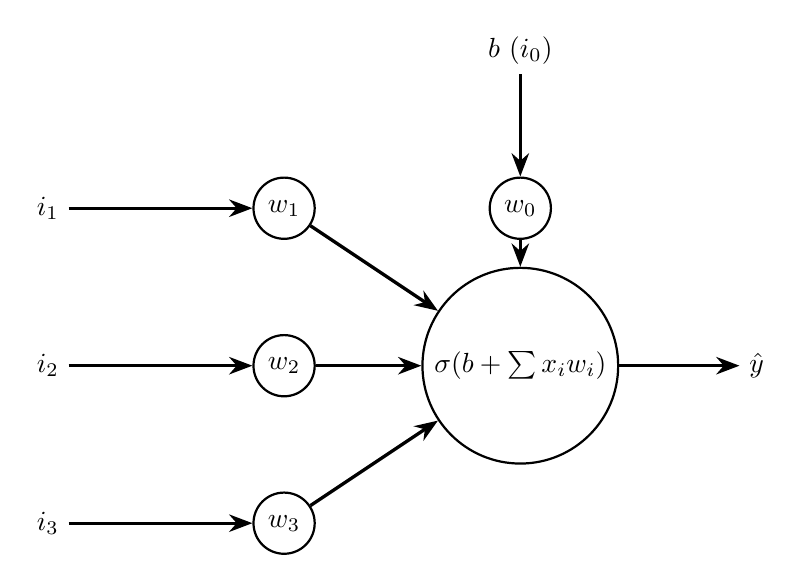
\begin{tikzpicture}
        \begin{scope}
            \node (i1)[empty-node] at (0,2) {$i_1$};
            \node (i2)[empty-node] at (0,0) {$i_2$};
            \node (i3)[empty-node] at (0,-2) {$i_3$};
            \node (b)[empty-node] at (6,4) {$b$ ($i_0$)};
            \node (w0)[weight-node] at (6,2) {$w_0$};
            \node (w1)[weight-node] at (3,2) {$w_1$};
            \node (w2)[weight-node] at (3,0) {$w_2$};
            \node (w3)[weight-node] at (3,-2) {$w_3$};
            \node (y)[empty-node] at (9,0) {$\hat{y}$};
            \node (f)[op-node] at (6,0) {$\sigma(b + \sum x_iw_i)$} ;
        \end{scope}

        \begin{scope}[>={Stealth[black]}, every edge/.style=black-line]
            \path [->] (b) edge node {} (w0);
            \path [->] (i1) edge node {} (w1);
            \path [->] (i2) edge node {} (w2);
            \path [->] (i3) edge node {} (w3);
            \path [->] (w0) edge node {} (f);
            \path [->] (w1) edge node {} (f);
            \path [->] (w2) edge node {} (f);
            \path [->] (w3) edge node {} (f);
            \path [->] (f) edge node {} (y);
        \end{scope}

    \end{tikzpicture}
\end{document}
